\documentclass[a4paper,11pt]{article}
\usepackage{pos}
\usepackage{siunitx}
\RequirePackage{orcidlink}
%
\usepackage{lineno} % for line numbers
\linenumbers % for line numbers
%
\title{Physics objects validation at the High-Level Trigger reconstruction in CMS}
%
\author[a]{Bruno Alves\orcidlink{0000-0001-9752-0624}\footnote{Copyright 2026 CERN for the benefit of the CMS Collaboration. Reproduction of this article or parts of it is allowed as specified in the CC-BY-4.0 license.}}
%
\affiliation[a]{CERN, 1211 Geneva 23, Switzerland}
%
\emailAdd{bruno.alves@cern.ch}
%
\newcommand{\sm}{\ensuremath{\sim}}
%
\abstract{As part of CERN’s Next Generation Triggers (NGT) project, the R³ (Real-time Reconstruction Revolution) program aims to rethink how the High-Level Trigger (HLT) event reconstruction is performed within the CMS Collaboration.
A key objective of R³ is to ensure an accurate and robust reconstruction, validating the quality of physics objects measured during data-taking at the upcoming High-Luminosity LHC.
This contribution presents our latest efforts to develop robust validation tools for the HLT community in CMS, as new, untested, and heterogeneous algorithms are rapidly developed and deployed.
We detail the tools and observables defined and measured for jets, missing transverse energy (MET and MHT), and Particle Flow objects, which are essential for comparing detector configurations across different phase-space regions.
We outline the metrics established to validate all objects, including efficiencies, fake rates, responses, and resolutions.
Furthermore, we demonstrate how these tools have already improved the reconstruction of certain objects, fostering collaboration with relevant experts.
Finally, we highlight the potential for these tools to also benefit the offline reconstruction, given some similarities with the HLT.
}
%
\FullConference{43rd International Conference on High Energy Physics (ICHEP 2026)\\
30 July to 5 August, 2026\\
Natal, Brazil\\}
%
\begin{document}
\maketitle
%
\section{The Status of the CMS Trigger System and NGT Scouting Validation Tools}
\label{intro}
%
The CMS experiment at the LHC~\cite{cms} employs a two-tiered online selection system: the hardware-based Level-1 Trigger (L1T), operating within a \SI{12.5}{\micro\second} latency budget, and the software-based High-Level Trigger (HLT)~\cite{hlttdr}, with a \SI{1}{\second} latency allowance. Together, these systems reduce the \SI{40}{\mega\hertz} bunch-crossing rate to an affordable data-recording volume.
To circumvent computing and storage bottlenecks, CMS pioneered \textit{data scouting}, which reconstructs events at the HLT level and outputs a streamlined, analysis-ready format without retaining raw detector data for full offline reconstruction.
To meet the demands of the High-Luminosity LHC (HL-LHC) era, the Next-Generation Triggers (NGT) project~\cite{ngt} expands this paradigm with a novel NGT Scouting stream (Fig.~\ref{fig:concept}) designed to process and record \emph{all} L1T-accepted events at a rate of \SI{750}{\kilo\hertz} in a compact, \texttt{NanoAOD}-like format, substantially exceeding the baseline HL-LHC scouting target of \SI{225}{\kilo\hertz} and the standard HLT raw-data rate of \sm\SI{15}{\kilo\hertz}~\cite{octdr}. \par
%
Current validation tools available in CMS are scattered, occasionally outdated, and often incomplete.
NGT and HLT upgrade efforts demand a reliable and comprehensive validation of physics objects.
We aim to provide detailed monitoring of these HL-LHC developments by enabling systematic comparisons across CMS software releases, data conditions, algorithm versions, and algorithm configurations or tunings.
Our tools, described in Section~\ref{sec:valid}, are fully integrated within the CMS software and are automated through its Data Quality Monitoring service.
These efforts can also often be generalized to offline objects, due to their structural similarities.
%
\begin{figure}[h]
\centering
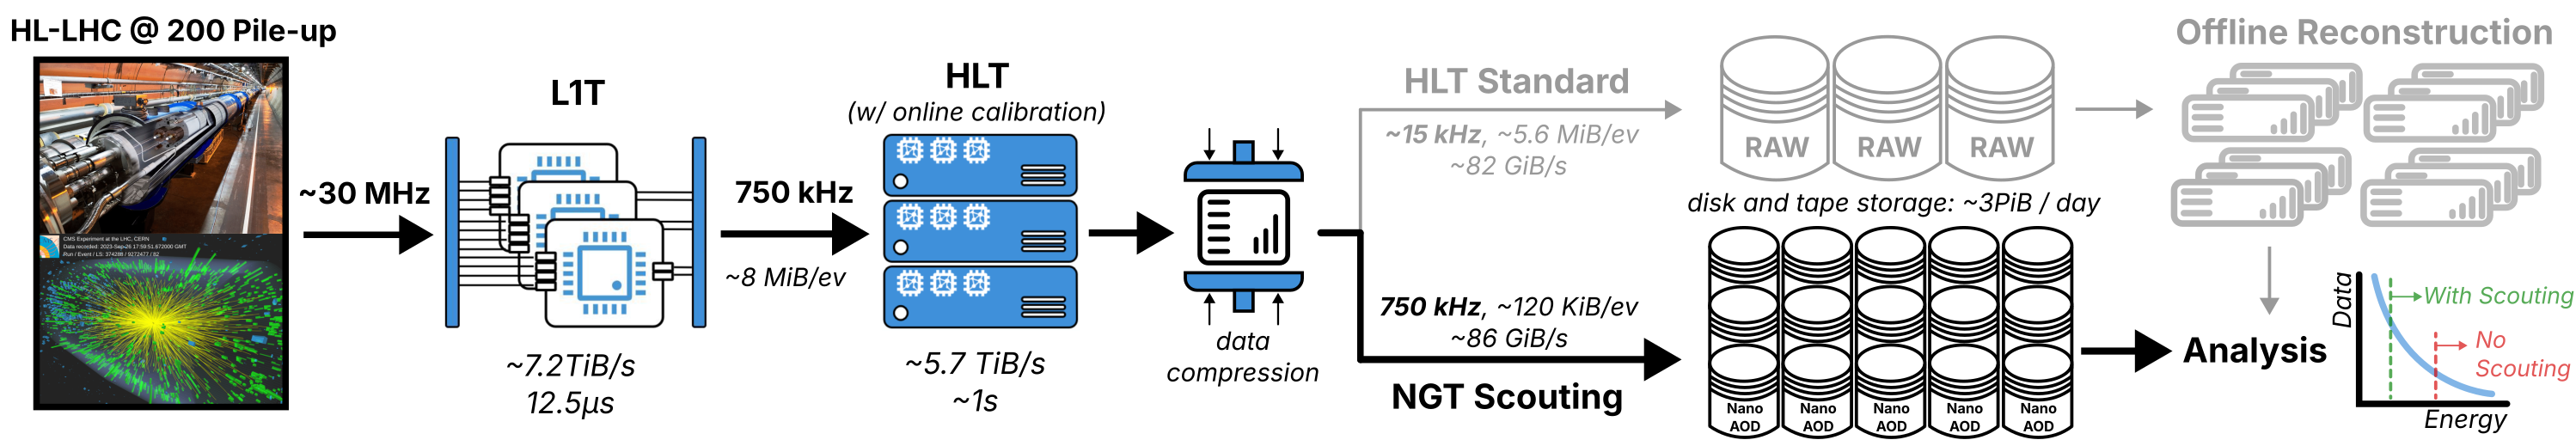
\includegraphics[width=1.\textwidth]{ngtconcept}
\caption{Simplified schematic overview of the trigger processing chain in CMS during Phase~2, from the collision rate at the HL-LHC with 200 pile-up to the final analysis step.
  Both the HLT Standard and the NGT Scouting paths are shown, with current expected rates and throughput values~\cite{octdr}.
  The HLT Standard approach selects high-interest events at \sm\SI{15}{\kilo\hertz} and writes out the full detector raw data for later offline analysis.
  The NGT Scouting path reconstructs all events accepted by the L1T at \SI{750}{\kilo\hertz}, with no additional filtering, and stores the events directly in a compact, analysis-ready \texttt{NanoAOD}-like data format.}
\label{fig:concept}
\end{figure}
%
\section{The Validation of Physics Objects}
\label{sec:valid}
To quantitatively evaluate physics object performance, the following metrics are defined:
\textit{Efficiency} measures the ratio of simulated objects matched to reconstructed ones over all simulated objects,
\textit{Fake Rate} quantifies the proportion of reconstructed objects not matched to any simulated object relative to all reconstructed objects,
\textit{Duplicate Rate} calculates the fraction of simulated objects matched to multiple reconstructed objects out of all simulated objects,
\textit{Merge Rate} determines the fraction of reconstructed objects matched to multiple simulated objects relative to all reconstructed objects,
\textit{Response} is the ratio between reconstructed and simulated energy or momentum, and
\textit{Resolution} is the standard deviation of the Gaussian curve fitting the response distribution. \par
%
A series of centralized validation tools have been recently developed at the HLT. 
\textbf{Particle Flow (PF) cluster} validation exploits hit-by-hit association logic between simulated truth and reconstructed information.
Current efforts focus primarily on PF clusters in the Electromagnetic Calorimeter (ECAL) to compare the physics performance of several clustering algorithms designed for the HL-LHC.
Custom ECAL event displays have been deployed to allow visual inspection of event topologies.
%
For measuring the performance of \textbf{secondary vertexing} algorithms, we consider the full set of simulated vertices including pile-up interactions, providing a reliable fake rate estimation.
The framework establishes a robust association to reconstructed vertices via tunable position and track-matching requirements.
This approach offers a flexible efficiency estimate that can be customized to different phase-spaces or decay types.
%
\textbf{Jet and MET/MHT} validation is indispensable to compare performance across different detector regions, jet algorithms, and hyperparameter configurations.
It has already been exploited to improve physics performance by identifying hidden pitfalls in new algorithms.
%
In \textbf{hadronic tau} validation, candidates are matched to generated visible taus using a spatial $\Delta \text{R}$ distance cut.
The DeepTauID tau tagger effectively reduces fakes originating from jets, while fake mitigation from background leptons is currently being integrated into the HLT framework.
%
Finally, \textbf{pixel track} validation provides simulation truth for intermediate objects within the pixel tracking algorithm, enabling an in-depth analysis of the efficiency across all intermediate objects.
This capability is especially relevant for Phase-2, where the number of tracking parameters grows into the hundreds.
The framework is also being leveraged to evaluate electron reconstruction.
%
\section{Conclusions}
\label{sec:conclusions}
%
We have developed essential validation tools tailored for monitoring Phase-2 detector and software upgrade efforts, which actively enable and motivate detailed performance studies and further algorithm developments. Work is currently ongoing to extend both the hadronic tau and MET/MHT validation frameworks. Looking forward, we plan to continue Particle Flow validation efforts by expanding to Hadronic Calorimeter (HCAL) clusters and eventually to full PF candidates. These ongoing and future efforts will benefit significantly from a comprehensive truth-graph, containing the full simulated event history, currently under development.
%
\begin{thebibliography}{99}
\bibitem{cms}
  The CMS Collaboration. ``The CMS Experiment at the CERN LHC''. In: JINST 3 (2008), S08004. DOI: \url{https://doi.org/10.1088/1748-0221/3/08/S08004}.
\bibitem{hlttdr}
  The CMS Collaboration. ``The Phase-2 Upgrade of the CMS Data Acquisition and High Level Trigger''. \url{https://cds.cern.ch/record/2759072/}.
\bibitem{ngt}
  Next Generation Triggers. ``NGT Evaluation Report - 2025. CERN''. DOI: \url{https://doi.org/10.17181/dvqah-g0f70}.
\bibitem{octdr}
  The CMS Collaboration. ``CMS Offline Software and Computing for HL-LHC, Conceptual Design Report''. \url{https://cds.cern.ch/record/2957472}.
%% \bibitem{cmstruthdocs}
%%   F. Pantaleo et al. ``CMS MC-truth graph (documentation)''. \url{https://github.com/felicepantaleo/cms-truth-docs}
\end{thebibliography}
%
\end{document}
